\documentclass[12pt,a4paper]{report}
%设置页面
\usepackage[top=1in,bottom=1in,left=1.25in,right=1.25in]{geometry}
\usepackage{graphicx}
\usepackage[pagestyles,indentafter]{titlesec}
\usepackage{fontspec,xunicode,xltxtra}
\titleformat{\section}{\Large}{\thesection}{1em}{}
\XeTeXlinebreaklocale "zh"
\XeTeXlinebreakskip = 0pt plus 1pt minus 0.1pt

\titleformat{\chapter}[hang]{\centering\LARGE\bfseries}{\chaptername}{1em}{}
%定义字体
\newfontfamily\kai{Adobe Kaiti Std}
\newfontfamily\msyh{微软雅黑}
\newfontfamily\fsong{Adobe Fangsong Std}
\newfontfamily\song{Adobe Song Std}
\newfontfamily\hei{Adobe Heiti Std}
\newfontfamily\mono{Droid Sans Mono}
%%%%%

\usepackage{listings} %列出代码%
\usepackage{xcolor} %列出代码%
%\lstset{language=Ruby ,label=ruby,backgroundcolor=\color{gray!50},frame=shadow,breaklines=true,basicstyle=\small,numbers=left,numbersep=1pt}
\lstset{language=Ruby ,label=ruby,backgroundcolor=\color{gray!50},frame=shadow,breaklines=true,basicstyle=\small}


% 代码边框设置 %


%%%
\renewcommand{\chaptername}{\msyh 第\thechapter 章}

\renewcommand{\baselinestretch}{1.38}



\begin{document}
\newpagestyle{main}{
    \sethead{}{}{\kai\small\chaptername\quad\chaptertitle\qquad\thepage}
    \setfoot{}{}{\thepage}\headrule\footrule}

\song
\title{\msyh puppet 入门}
\author{huangmingyou@gmail.com}

\maketitle
\renewcommand{\contentsname}{目录}
\tableofcontents


\pagestyle{main}
\newpage
\begin{center}
\msyh 前言
\end{center}
\fsong
\par
随着数据中心服务器的增加,传统的系统维护方法有点捉襟见肘,于是出现了配置管理软件,利用配置管理,可以把整个数据中心的服务器的所有配置内容管理起来,方便大规模的管理以及快速的部署。配置管理软件有很多,最出名的是cfengine,但是cfengine的语法比较晦涩,于是出现了puppet  。puppet的语法简单,对管理内容的抽象很好,很容易理解代码,因此最近正迅速的流行开来。puppet是免费开源软件。可以自由使用,现在 google正使用puppet管理超过6000台的mac桌面电脑。这还是07年的数据。 另外很多世界知名的it企业也在使用puppet,开源社区的fedora也使用puppet。国内的大公司也在准备从cfengine转移到puppet上面。\par
撰写本文的目的是让初学者对 puppet有一个简单的认识能快速的入门,因为是利用空余时间完成,时间和精力有限,因此只讲解了最基本的内容,高级的内容都没讲解,如果你需要深入学习可以参考国内的中文 wiki 以及官方的文档。\par
本文欢迎转载,但是请保留作者信息。\par
本手册的最新版本可以从:http://code.google.com/p/puppet-manifest-share/downloads/list 获得。
\song
\newpage
\chapter{\msyh puppet简介}
\begin{center}
\kai
\small
滚滚长江东逝水,浪花淘尽英雄。是非成败转头空。\\
青山依旧在,几度夕阳红。 \\
白发渔樵江渚上,惯看秋月春风。一壶浊酒喜相逢。\\
古今多少事,都付笑谈中。\footnote{\fsong \tiny puppet被认为是下一代的cfengine,cfengine是一个老牌的配置管理软件}
\end{center}

\song
\section{\msyh puppet是什么}

puppet\footnote{\fsong\tiny 最开始是由luke开发的开源软件,现在开始公司化运作,但是软件依然是开源和免费的}是一个为实现数据中心自动化管理而设计的配置管理软件。基于c/s架构。puppet的服务器端保存着所有的对客户端服务器的配置代码,在puppet里面叫做manifest. 客户端下载manifest之后,可以根据manifest对服务器进行配置,例如软件包管理,用户管理和文件管理等等。
\par
这样就把日常的系统管理任务代码化了,代码化的好处是可以分享,保存,避免重复劳动,也可以快速恢复以及快速的大规模部署服务器。同时,manifest可以的根据客户端服务器的配置情况(硬件和软件)来动态生成。
\begin{center}
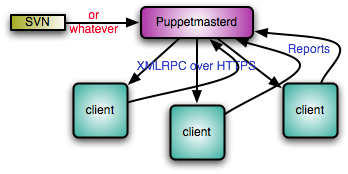
\includegraphics[width=0.6\textwidth]{Puppet_Star.png}
\end{center}


\par
在Unix/Linux系统管理的内容上面,通常就是管理软件包,用户,文件内容以及crontab等。在puppet的世界里面,这些内容都被看作是”资源“,每种资源都有对应的属性,例如软件包有安装和不安装的属性,文件有权限属性。puppet的代码主要就是由这些资源和资源的属性构成。
\par
为了快速的开始入门,建议你手上有一个可以随时使用的debian或者ubuntu系统,方便快速安装puppet软件。装一个虚拟机是一个不错的选择。\par

\section{\msyh Hello world}
puppet有两种执行模式,一是直接运行puppet file.manifest 二是puppetd --server puppetmaster.server.com;前面一种是直接读取file.mainfest文件进行配置,后一种是从服务端下载manifest进行配置。为了先对puppet的资源概念有一个简单的认识,下面将给出一个直接执行manifest的例子,看看manifest怎么去写。首先通过执行apt-get install puppet在系统上面安装好puppet客户端软件。然后编写一个manifest文件/tmp/1.pp,内容如下:
\msyh\small
\begin{lstlisting}
file {
      "/tmp/test":
        content=>"hello\n",
        mode => 0644;
        }
\end{lstlisting}
\song
然后执行 puppet  /tmp/1.pp ;执行完成以后,将会在/tmp目录下面生成一个文件test,文件内容是"hello";第一行的file表明是什么类型的资源,第二行的"/tmp/test"叫做这个资源的title;用来代表这个资源,后面两行设置这个资源的属性。\par
再来看一个例子:
\msyh
\begin{lstlisting}
package{
        ["gcc","make"]:
        ensure => installed;
}
\end{lstlisting}
\song
这是配置一个包资源,包是gcc和make, 第三行是指定这两个包的属性,在这里是installed,表示要安装这两个软件包。
\msyh 再次提醒:不同的资源有不同的属性,但是又有一些属性是所有资源都共有的,例如tag,这种属性叫做元属性。
\song
\newpage



\chapter{\msyh puppet安装}
\begin{center}
\kai
兵马未动,粮草先行
\end{center}

\song 本章介绍puppet在各个linux发行版的安装,puppet的安装可以从源代码安装,也可以从二进制发行包安装,还可以从ruby的gem安装。下面分别介绍各种linux系统上最便捷的安装方法。顺便说一句,ruby\footnote{\fsong\tiny puppet的作者说当初选择了很多种开发语言,最后选择ruby是因为可以快速的开发并且满足他的需求}是puppet的开发语言。
\song
\section{\msyh debian 系发行版安装puppet}
debian或者ubuntu的软件仓库已经包含了puppet软件,(注:软件包的名字可能会因为系统升级而变化,请先用apt-cache搜索一下),在安装软件之前先设置好主机名,因为puppet要使用ssl证书,证书包含主机名,修改主机名\footnote{\fsong\tiny 其他linux系统修改的方法可能会不一样}首先编辑/etc/hostname,然后执行hostname -F /etc/hostname; 主机名修改后重新登录系统。用下面的命令安装puppet。
\msyh
\begin{lstlisting}
apt-get install puppet puppetmaster
\end{lstlisting}
\song
这样就安装好了客户端和服务器端的软件。

\section{\msyh redhat 系发行版安装puppet}

centos的官方软件库里面不包含puppet包,但是在epel项目里面有包含puppet包. epel 是一个对rhel软件仓库的扩展,把一些有用的,但是rhel库没包含的软件收集在一起做成的一个软件仓库.
因此首先在centos上面安装epel,以 32位的centos5 举例,其他版本以此类推
\msyh
\begin{lstlisting}
rpm -Uvh http://download.fedora.redhat.com/pub/epel/5/i386/epel-release-5-3.noarch.rpm
\end{lstlisting}
\song
安装好epel库以后,就可以用下面的命令安装puppet了
\msyh
\begin{lstlisting}
yum install puppet
\end{lstlisting}
\song
因为rhel没有yum 包管理系统,因此需要先安装yum软件,再按照上面的方法安装puppet,不在赘述.


\section{\msyh 源代码安装puppet}
首先从http://projects.reductivelabs.com/projects/puppet/wiki/Downloading\_Puppet 下载最新的puppet稳定(stable)版本和facter稳定版。
同时安装下面的依赖包
\msyh
\begin{lstlisting}
base64
cgi
digest/md5
etc
fileutils
ipaddr
openssl
strscan
syslog
uri
webrick
webrick/https
xmlrpc
\end{lstlisting}
\song
然后先安装facter
\msyh
\begin{lstlisting}
tar zxf facter-1.5.7.tar.gz
cd facter-1.5.7
ruby install.rb
\end{lstlisting}
\song
再安装puppet
\msyh
\begin{lstlisting}
tar zxf puppet-0.25.4.tar.gz
cd puppet-0.25.4
ruby install.rb
\end{lstlisting}
\song

\section{\msyh 配置c/s模式的puppet试验环境}
工欲善其事,必先利其器!本节讲解如何配置c/s结构的puppet测试环境,生产环境也这样配置。首先准备两台虚拟主机,安装debian或者ubuntu系统。两台主机的主机名分别设置成client.puppet.com和server.puppet.com,参考前面的方法设置好主机名以后再安装puppet软件。以后用client.puppet.com代表客户端,用server.puppet.com代表服务器端。\par
请参考下面的步骤操作,这里选用debian和规定好主机名,是尽量减少初学者的麻烦。debian版本是5.1。\par
首先,在客户端安装puppet软件\par

\msyh
\begin{lstlisting}
apt-get install puppet
\end{lstlisting}
\song

然后在服务器端安装puppetmaster软件

\msyh
\begin{lstlisting}
apt-get install puppetmaster
\end{lstlisting}
\song
在客户端的/etc/hosts里面添加服务器的解析,例如:
\msyh
\begin{lstlisting}
echo "192.168.0.10 server.puppet.com" >>/etc/hosts
\end{lstlisting}
\song

puppet的客户端和服务器是通过ssl链接的,在服务器有一个自签名的根证书,在安装软件的时候自动生成。\msyh 注意:要在安装软件以前先设置主机名,因为生成证书的时候要把主机名写入证书,如果证书生成好了再改主机名,就连不上,这是很多初学者遇到的问题。\song 每个客户端的证书要经过根证书签名才能和服务器连接。所以首先要在客户端执行下面的命令来请求服务器签名证书。

\msyh
\begin{lstlisting}
puppetd --test --server server.puppet.com
\end{lstlisting}
\song
执行上面的命令,客户端将生成证书,并且把证书签名请求发到服务器端。登录到服务器端,执行下面的命令查看是否有客户端的证书请求:
\msyh \begin{lstlisting}
pupetca --list
\end{lstlisting} \song
如果看到了客户端的证书请求,用下面的命令对所有证书请求签名:
\msyh \begin{lstlisting}
pupetca -s -a
\end{lstlisting} \song
这样,客户端和服务器端就配置好了,可以在服务器端配置好测试manifest代码进行测试。
puppetmaster的第一个执行的代码是在/etc/puppet/manifest/site.pp
因此这个文件必须存在,而且其他的代码也要通过代码来调用.
现在,建立一个最简单的site.pp文件,内容如下
\msyh \begin{lstlisting}
node default {
          file { "/tmp/temp1.txt": 
		content => "hello"; }
         }
\end{lstlisting} \song
上面的代码对默认连入的puppet客户端执行一个操作,在/tmp目录生成一个temp1.txt文件,内容是hello,first puppet manifest.
回到客户端,执行下面的命令:
\msyh \begin{lstlisting}
pupetd --test --server server.puppet.com
\end{lstlisting} \song
这样,客户端将会从服务器下载默认的执行代码,在/tmp目录下生成叫做temp1.txt的文件。



\chapter{\msyh puppet语法}
\begin{center}
\kai
磨刀不误砍柴功\par
\end{center}
\song
\par
本章简单介绍puppet的语法,因为puppet是用ruby编写的,因此puppet的语法也和ruby类似,都是很简单的面对对象的高级语言。再次强调,puppet把需要管理的内容抽象成为资源,每种资源有不同的属性,因此puppet语言就是描述这些资源的属性以及资源之间关系的语言。\par
\section{\msyh 资源}
定义一个资源,需要指定资源的类型和资源的title。看一个例子:
\msyh \begin{lstlisting}
file {
	"/etc/passwd":
	name => "/etc/passd",
	owner => root,
	group => root,
	mode => 644;
	
}
\end{lstlisting} \song
上面的代码让/etc/passwd的权限保持644,并且属于root用户和root用户组,file是指定资源的类型是 "file"类型,第二行的 "/etc/passwd"是资源的title, title的作用是让puppet能唯一标识这个资源。第三行的name指定了要对那个文件操作,默认情况下,name都等于title,所以很多时候name是可以省略的。这点要注意。看下面的例子 :
\msyh \begin{lstlisting}
file { 
"sshdconfig":
name => $operatingsystem ? {
	solaris => "/usr/local/etc/ssh/sshd_config",
	default => "/etc/ssh/sshd_config",
},
owner => root,
group => root,
mode  => 644,
}
\end{lstlisting} \song

资源的title是sshdconfig,但是name却可以通过判定操作系统自己选择合适的值。这样,当其他的资源要依赖sshdconfig的时候,只需要说明依赖sshdconfig就行,不需要关心文件到底在什么路径下面。
例如下面的代码:
\msyh \begin{lstlisting}
service { "sshd":
subscribe => File[sshdconfig],
}
\end{lstlisting} \song
指定了一个sshd的服务,这个服务如果发现文件资源 sshdconfig 有变动,就会自己reload配置文件。是不是很方便呢?注意上面的subscribe后面的File,第一个字母要大写,定义资源关系的时候,这里的字母要大写。
\par

通常,在puppet代码里面可能会定义很多相同的资源,可以用[]把所有资源的 title写在一起,例如:
\msyh \begin{lstlisting}
file{
	["/etc/passwd","/etc/hosts"]:
	owner => root,
	group => root,
	mode => 644;
}
\end{lstlisting} \song


你可能已经发现了,每次定义文件的时候如果都输入mode,owner,group会很繁琐,因此你可以在puppet的site.pp的开头定义资源的默认值。定义资源的默认值需要把资源的第一个资源大写。例如下面的代码让所有的file资源的mode是644,owner是root。
\msyh \begin{lstlisting}
File{ owner => root, mode => 644 ;}
\end{lstlisting} \song
默认值可以被后面的设置覆盖。
\par

在puppet里面可以定义资源之间的关系,例如前面提到的,如果sshdconfig文件如果有修改,sshd服务就重启。puppet里面还有另一个资源关系,依赖。例如资源A依赖资源B,如果资源B不存在,资源A就不被执行。定义资源依赖的属性是 requre 。例如 :
\msyh \begin{lstlisting}
file { 
      "/etc/apache2/port.conf":
	content => "80",
	require => Package["apache2"];
	}
package{
	"apache2":
	ensure => installed;
	}
\end{lstlisting} \song

file资源设置port.conf的内容为80,但是在设置file资源之前,要求apache2这个软件包配置好了。

\section{\msyh 类和函数}
类的作用是把一组资源收集在一个盒子里面,一起使用,例如把sshd和他的配置文件做成一个ssh类,其他的地方要用到就直接包含ssh类就可以了,方便写出更简洁的代码,便于维护。类可以继承。看一个具体的例子:
\msyh \begin{lstlisting}
class ssh{
	file { 
		"/etc/ssh/sshd_config":
		source => "puppet://$fileserver/ssh/sshd_config.cfg";
		}
	package { 
		"ssh":
		ensure => installed;
	}
	service {
		"ssh":
		ensure => running;
	}
}
\end{lstlisting} \song
这里,file /etc/ssh/sshd\_config的内容是从puppet服务器上面下载的,file资源的内容可以从别的url得到,也可以erb模板生成,erb模板是很强大的工具,这个后面会说到。package资源安装ssh软件,service资源保证ssh服务在运行状态。类的继承这里就不讲了,因为是入门手册,另外用的不多。
\par
puppet的官方文档里面是没有puppet函数这一说法的,而是叫做define ; 这里我写做函数,是因为define实现的功能其实和函数一样,而且在ruby里面也是用define来定义一个函数。这里写做函数,便于理解。\par
具体来看一个例子:
\newpage
\msyh \begin{lstlisting}
define svn_repo($path) {
    exec { 
	"/usr/bin/svnadmin create $path/$title":
        unless => "/bin/test -d $path",
    }
}

svn_repo { 
	puppet_repo: 
	path => "/var/svn_puppet" }
svn_repo { 
	other_repo:  
	path => "/var/svn_other" }
\end{lstlisting} \song


首先用define定义了一个svn\_repo函数,并且带了一个参数\footnote{\fsong\tiny  因为可以带参数,所以我觉得翻译成函数更好} 。这个参数可以在函数里面的资源使用,在这里,exec资源根据提供的参数创建 svn 仓库。函数定义好以后,后面的两行就用定义好的函数创建了两个svn库。相信聪明的你已经完全明白了类和函数怎么用了吧\footnote{\fsong\tiny 注意看函数的使用语法,是不是和使用资源一样,path可以看作是属性},那就不在赘述。


\par
\section{\msyh 节点}
puppet如何区分不同的客户端,并且给不同的服务端分配manifest呢?puppet使用叫做node的语法来做这个事情,node 后面跟客户端的主机名\footnote{\fsong\tiny 主机名在puppet里面很重要},例如下面的例子:
\msyh \begin{lstlisting}
node 'host1.example.com' {
	include ssh
	}
node 'host2.example.com' {
	include apache,mysql,php
	}
\end{lstlisting} \song

当主机host1.example.com来连服务端时,只会执行node 'host1.example.com'里面的代码,不会执行node host2.example.com里面的代码。正如前面所说,可以定义一个default结点。比如没有针对host3的node配置,host3就用default的配置了。在这里include的意思是include 类。同样,节点也支持继承,同样,也不打算深入。\par
使用节点的时候,尽量把所有的配置写成类,节点里面定义好变量和包含相应的类就可以了。保证代码的简洁。例如:
\msyh \begin{lstlisting}
node 'host4.example.com' {
	$networktype="tele"
	$nagioscheckport="80,22,3306"
	include ssh,apache,mysql
}
\end{lstlisting} \song

\section{\msyh 变量和数组 }

puppet也和其他语言一样,支持变量和数组,puppet用\$符号定义变量,变量的内容用双引号括起来。例如 :
\msyh \begin{lstlisting}
$test="hello,guys"
file {
	"/tmp/test":
	content => $test;
}
\end{lstlisting} \song

puppet可以使用由facter提交的变量,facter在客户端收集系统信息整理成不同的变量提交给puppet服务器端,服务器端的代码可以使用这些变量实现高级的功能,例如不同的硬件配置生成不同的应用软件配置文件。 运行facter命令可以看到很多变量的输出,这些变量可以在puppet代码里面直接使用。\par
puppet利用方括号来定义数组,数组的内容由逗号分割,例如下面的例子:
\msyh \begin{lstlisting}
["apache2","httpd","ssh"]
\end{lstlisting} \song

数组可以用在资源定义里面,例如前面提到的例子。也可以用在函数里面,例如:
\msyh \begin{lstlisting}
define php::pear() {
    package { "`php-${name}": ensure => installed }
}

php::pear { ['ldap', 'mysql', 'ps', 'snmp', 'sqlite', 'tidy', 'xmlrpc']: }
\end{lstlisting} \song


变量也有有效范围,同其他语言一样分为局部和全局变量,简单说来,就是在{}里面定义的变量的使用范围就限制在{}里面。
同时,puppet还简单的支持 if ... eles 语法,但是用的不多,不在深入。

\section {\msyh 模块}
简单来说,一个模块就是一个/etc/puppet/modues目录下面的一个目录和它的子目录,在puppet的主文件site.pp里面用import modulename可以插入模块。新版本的puppet可以自动插入/etc/puppet/modues目录下的模块。引入模块,可以结构化代码,便于分享和管理。例如关于apache的所有配置都写到apache模块下面。一个模块目录下面通常包括三个目录,files, manifests,templates 。manifests 里面必须要包括一个init.pp的文件,这是该模块的初始文件,导入一个模块的时候,会从init.pp开始执行。可以把所有的代码都写到init.pp里面,也可以分成多个pp文件,init 再去包含其他文件。\par
files目录是该模块的文件发布目录,puppet提供一个文件分发机制,类似rsync的模块,后面详细介绍。templates 目录包含erb模型文件,这个和file资源的template属性有关,后面详细介绍。 \par
puppet安装好以后,modules目录是没有的,自己建立一个就行,然后在里面可以新增加你的模块。请养成使用模块的习惯。


\chapter{\msyh 几个常用的资源}
\begin{center}
\kai
不入虎穴,焉得虎子
\end{center}
\par
puppet提供了很多资源类型,但是常用的就那么几个。在讲解具体的内容之前,先了解一下provider这个概念,puppet管理不同的资源,是利用不同的provider来管理的。例如管理package资源,在debian上面是用的apt-get,在redhat上面是用的yum 。在这里,apt,yum就是provider。在定义资源的时候,可以明确指定provider。但是通常都是由puppet自己探测。因为不同的provider功能不一样,所以在不同的操作系统上面,有些资源能实现的功能也不一样,例如在linux上面设置user资源的时候,不能设置密码(新的puppet或许已经支持),需要用其他辅助手段来完成,但是设置 ldap用户的时候是可以设置密码的。
\section{\msyh file资源}
file资源在puppet里面用的挺多,属性包括大家已经属性的owner,group,mode,content等等。file还有两个重要的命令,。source和template.通常,一个文件的内容可以由content属性来包含固定的内容,但是也可以用source命令来从其他url复制文件内容。目前puppet只支持puppet这个url,表示从puppet的fileserver去下载文件内容。例如:
\msyh \begin{lstlisting}
source => "puppet://${fileserver}/lvs/${corp}.${idc}.keepalived.conf"
\end{lstlisting} \song
其中fileserver后面的lvs表示是lvs模块的files目录这个路径。正如前面提到的一样。用 source就可以把很多配置文件放到puppet服务器端统一管理。

file资源的另一个template命令是一个功能强大的命令。利用template,可以通过erb模板生成文件内容,erb模板可以使用变量。而且还可以对变量进行计算和操作。这是puppet强大的地方,举一个例子,你配置两台squid服务器,两台服务器的内存不一样,那么在squid.conf里面有关内存的配置命令就要根据硬件配置来设置。在过去,你只能手工去判定和修改,现在puppet自己搞定。看下面的代码:
\newpage
\msyh \begin{lstlisting}
file {
	"/etc/squid/squid.conf":
	mode => 0644,
	content => template ("squid/squid.conf.erb");
}
\end{lstlisting} \song

这里的template里面的"squid/squid.conf.erb"表示的路径是squid模块下面templates目录下的squid.conf.erb这个路径。
看看squid.conf.erb里面的部分内容\footnote{\fsong\tiny vmx\_memsize 和 fqdn 是facter提交的变量,表示内存和主机名}

\msyh \begin{lstlisting}
cache_mem <%= Integer(vmx_memsize.to_i*0.45) -%> MB
visible_hostname <%= fqdn %>
\end{lstlisting} \song
在这里,cache\_mem设置成总内存的45\%大小,visible\_hostname 设置成主机名。更多有趣的功能也可以实现。
\section{\msyh package资源}
package资源管理系统的软件包安装,该资源的主要属性是ensure;设置该软件包应该在什么状态. installed 表示要安装该软件,也可以写成present; absent 表示反安装该软件,pureged 表示干净的移除该软件,latest 表示安装软件包的最新版本.例如:
\msyh \begin{lstlisting}
package {
    ["vim","iproute","x-window-system"]:
    ensure => installed;
    ["pppoe","pppoe-conf"]:
    ensure => absent;
    }
\end{lstlisting} \song
安装vim等包,删除pppoe,pppoe-conf包。如果你的系统安装的是编译的软件包,建议你打包成操作系统的包格式,建立你自己的软件仓库。
\section{\msyh service资源}
service资源表示保证/etc/init.d目录下的服务执行脚本执行什么命令,例如:
\msyh \begin{lstlisting}
service {
	"ssh":
	ensure => running;
	"nfs":
	ensure => stoped;
}
\end{lstlisting} \song
puppet只保证服务会运行或者停止,但是不保证开机启动的服务的初始状态,既不会去管理/etc/rcX.d目录下的服务的链接。
service可以通过start,retart,status命令来指定这些命令的路径。如果不指定restart路径,当执行重启的时候就是先 stop再start服务。另外你还可以用pattern属性来设置搜索进程列表的匹配字符串,用于不支持init脚本的系统.当要停止一个服务的时候,通过查看进程运行列表来判断.

\section{\msyh exec资源}
exec资源在不到万不得已的时候不要去用,简单说来exec资源就是在执行puppet的时候,调用shell执行一条shell语句,例如:
\msyh \begin{lstlisting}
exec {
	"delete config":
	path => "/bin:/usr/bin",
	command => "rm /etc/ssh/ssh_config";
}
\end{lstlisting} \song
exec可以用path指定命令执行的预搜索路径,create属性表明该exec将创建一个文件,当下一次puppet执行的时候,如果发现了这个文件,就不再执行这个exec资源。\par
exec资源是不太好掌控的资源,如果能用脚本实现,尽量写成脚本通过file资源分发到服务器上面。然后用其他的方式来调用脚本。例如crontab。说来crontab资源,罗嗦一句,虽然puppet提供了crontab资源,但是你完全可以用file资源来把 crontab任务放到 /etc/cron.d目录下来实现crontab资源的管理。使用puppet的时候,尽量用最简单的语法,越是花哨的语法也越容易出错。


\chapter{\msyh puppet高级内容}
\begin{center}
\kai
欲穷千里目,更上一层楼
\end{center}
\par
puppet在大规模的生成环境中,如果只有一台puppetmaster,会忙不过来的,因为puppet是用 ruby写的,ruby是解析型语言,每个客户端来访问,都要解析一次,当客户端多了就忙不过来,所以需要扩展成一个服务器组。puppetmaster可以看作一个web服务器,实际上也是由ruby提供的web服务器模块来做的。因此可以利用web代理软件来配合puppetmaster做集群设置。这方面的资料在官方网站有详细介绍,例如puppet+nagix等等。\par
puppet后台运行的时候,默认是半小时执行一次,不是很方便修改。可以考虑让 puppetd 不运行在后台,而使用crontab来调用,执行完毕就退出,这样可以精确的控制所有的puppetd客户端的执行时间,分散执行时间也可以减轻puppetmaster服务器的压力。\par
puppet还支持外部资源,所谓外部资源,就是发布在客户端以外的资源,所有客户端都可以共享这些资源。\par
最后来看看puppet的工作细节,分为下面几个步骤:\par
一.客户端puppetd 调用facter, facter探测出主机的一些变量,例如主机名,内存大小,ip地址等。 pupppetd 把这些信息通过ssl连接发送到服务器端。\par
二.服务器端的puppetmaster 检测客户端的主机名,然后找到 manifest里面对应的 node 配置, 然后对该部分内容进行解析,facter送过来的信息可以作为变量处理,node牵涉到的代码才解析,其他没牵涉的代码不解析。 解析分为几个阶段,语法检查,如果语法错误就报错。\par
如果语法没错,就继续解析,解析的结果生成一个中间的“伪代码”,然后把伪代码发给客户端。\par
三.客户端接收到“伪代码”,并且执行,客户端把执行结果发送给服务器。\par
四.务器端把客户端的执行结果写入日志。\par


\chapter{\msyh puppet生产环境部署经验}
\begin{center}
\kai
古人学问无遗力,\\
少壮工夫老始成。 \\
纸上得来终觉浅,\\
绝知此事要躬行。 \\
\end{center}

通常,在生产环境部署puppet,一般是用c/s模式,部署一个或者一组puppetmaster。随着机器的增加,puppetmaster的负载会成为一个问题。本章我将描述一下我自己在生产环境的部署经验。不利用c/s模式来执行代码。而是利用客户端自行下载代码来解决负载问题。\par



\chapter{\msyh FAQ}
\par
\msyh Q: puppet的证书机制 \par
A: \song puppet证书问题是初学者最容易遇到的问题,这里讲一下怎么处理.puppet服务器端在安装或者首次启动的时候,会自动生产一个根证书和服务器证书,证书和主机名相关,因此如果证书生成后友改了主机名,那就会出问题.  puppet客户端在首次启动的时候,也会自动生成证书;但是这个证书需要得到puppet服务器端的签名才行,因此;puppet客户端第一次连接服务器的时候,会发送一个证书请求 ; 服务器端需要对这个证书进行签名. puppet客户端在下次连接服务器的时候就会下载签名好的证书.\par
\msyh Q:debian下面的证书出错,怎么解决?\par
A:\song 本方法是提供给初学者的测试环境,生成环境不建议这么做.首先在puppetmaster(服务器端)删除/var/lib/puppet/ssl目录;然后启动puppetmasterd ; 然后在客户端也删除/var/lib/puppet/ssl目录.把puppetmaster机器的主机名和对应的ip地址写入客户端机器的/etc/hosts. 然后执行
\msyh \begin{lstlisting}
puppetd --test --server server.example.com  #发送证书请求
\end{lstlisting} \song
 把server.example.com替换成你自己的服务器主机名. 执行这个命令,会有提示信息,不用理会.\par
然后登录到puppetmaster服务器机器,执行
\msyh \begin{lstlisting}
puppetca --list #列出所有证书请求
\end{lstlisting} \song
命令,看看是否有客户端的证书请求 ;如果没有,请检查前面的步骤是执行正确,以及网络连接是否正常. 如果puppetca --list 能看到请求,那么执行
\msyh \begin{lstlisting}
puppetca -s -a  #签名所有证书
\end{lstlisting} \song
命令 ; 对所有的证书请求签名.  \par
最后回到puppet客户端机器,执行
\msyh \begin{lstlisting}
puppetd --test --server server.example.com  #得到证书
\end{lstlisting} \song
就能建立连接了,如果你的site.pp写好了.就可以测试puppet了.\par
补充: 如果客户端和服务器端的时间不一致也会导致证书认证失败,因此出现证书问题的时候需要检查两台机器的时间是否一致,如果不一致用date命令或者ntpdate命令让两台机器的时间一致。\par

\msyh Q:redhat下面的证书问题如何解决? \par
A:\song 同debian ; ssl目录也是在/var/lib/puppet/ssl \par

\msyh Q:源代码安装的puppet如何解决证书问题? \par
A: \song 同debian,但是ssl目录在/etc/puppet/ssl \par

\msyh Q:如何配置puppetrun \par
A: \song 在puppet客户端建立一个文件/etc/puppet/auth.conf ,增加两行内容\par
\msyh \begin{lstlisting}
path /
allow *
\end{lstlisting} \song

然后用下面的参数启动puppetd,便于调试。
\msyh \begin{lstlisting}
puppetd --no-client --listen --verbose --no-daemonize --server server.puppet.com
\end{lstlisting} \song
启动好以后,用ss -nlp|grep puppet 命令看看puppetd是否监听到了8139端口。如果正常,在其他机器上运行
\msyh \begin{lstlisting}
puppetrun  --host host1.puppet.com 
\end{lstlisting} \song
命令来看看puppetrun是否正常。




\newpage
\begin{center}
\msyh
后记
\end{center}
\fsong
\par
本着学习tex,以及整理资料,推广puppet的目的,利用空余时间编写该入门文章,内容简单,水平有限,如果发现错误和错字请提醒我更改。\par
使用puppet也有点时间了,但是一直没有发现有好的中文资料,因此2010年年初建立了puppet.wikidot.com的免费的 wiki,翻译puppet的中文文档,还是因为英语水平有限,所以水准不高,所以有兴趣的朋友可以加入翻译。现在wiki已经列入了官方的wiki目录。目前puppet的其他语言翻译只有中文和日文。本文可以自由转发,请不要用于商业目的,对于该行为我表示强烈抗议,并且保留动手的权利。\par
在翻译的过程中,下列网友也加入了翻译,排名不分先后(wiki加入时间)。\par

\msyh \begin{lstlisting}

huangmingyou	
houqp	
frostynova	
aaniao999	
kuuyee	
edison7500	
min xu	
270175100	
douzl	
Daniel Ho	
unline	
wtoppp	
xw2014	
chifeng	
dywer	
Liu Nan	
\end{lstlisting} \song

\newpage
\begin{center}
\msyh
修改日志
\end{center}
\fsong


2010-12-07:	更新FAQ,时间问题也会导致证书认证失败。\par
2010-12-30:	更新FAQ,增加puppetrun的配置
2011-9-22:	修改几个拼写错误




\end{document}
